\documentclass[a4paper, 12pt]{article}

\usepackage[utf8]{inputenc}
\usepackage[T1]{fontenc}
\usepackage{verbatim}
\usepackage{graphicx}
\usepackage{setspace}
\usepackage{listings}
\usepackage{anysize}

\onehalfspacing

\usepackage{hyperref}
\hypersetup{
	pdftitle = {Databases - Facepalm}
	,pdfauthor = {Alexandre Santos \& João Ferreira \texttt{{acs, jpbat}@student.dei.uc.pt}}
	,pdfsubject = {Facepalm}
	,pdfkeywords = {RMI} {Java} {Facepalm} {Tomcat} {Apache} {Servlet} {JSP} {JavaBean} {WebSocket} {PostgreSQL} {Databases}
	,pdfborder = {0 0 0}
}

\title{Databases\\Facepalm}
\author{Alexandre Santos \& João Ferreira\\
		Department of Informatics Engineering\\
		University of Coimbra\\
		\texttt{acs@student.dei.uc.pt | jpbat@student.dei.uc.pt}\\
		\texttt{2009127404 | 2009113274}}
\date{December 2012}

\marginsize{3.5cm}{3.5cm}{3cm}{3cm}

\makeatletter

\begin{document}
\maketitle

\begin{figure}[h]
	
\includegraphics[keepaspectratio=true, height=0.475\textheight]{cover}
\end{figure}

\cleardoublepage

\tableofcontents
\cleardoublepage

\setlength{\parindent}{1cm}
\setlength{\parskip}{0.3cm}

\section{Introdução}
\indent \indent No desenrolar do projecto da cadeira Bases de Dados do 3º ano da Licenciatura em Engenharia Informática, foi-nos pedido que desenvolvessemos uma rede social. O seu desenvolvimento foi um processo de engenharia que foi desenvolvido ao longo de vários meses.

No ínicio foi-nos pedido que planeassemos sob que plataformas o trabalho iria ser desenvolvido, e quais as funcionalidades que iriamos implementar. Pediram-nos também que planeassemos tarefas em relação ao tempo que tinhamos disponível. No que diz respeito a isto muito pouco foi respeitado, uma vez que algumas cadeiras (nomeadamente Sistemas Distribuidos) nos deram mais trabalho do que inicialmente esperado, razão pela qual optámos por unir os 2 projectos. Assim o projecto foi desenvolvido usando Java 7, Apache Tomcat 7.0.37, PostgreSQL.

Na segunda meta foi-nos pedido um modelo ER da nossa base de dados. Este foi ligeiramente alterado, uma vez que as funcionalidades pedidas no projecto de Sistemas Distribuidos nos obrigaram a adicionar algumas entidades e adicionar alguns campos noutras.

A nossa primeira entrega funcional foi entregue em php pois tinha sido a nossa primeira previsão de linguagem de desenvolvimento do projecto, algo que como já expliquei acabou por ser abandonado, tendo sido todo o código migrado para a plataforma actual.
\cleardoublepage


\section{Apresentação}
\indent \indent Seja bem-vindo à Facepalm! Aqui nós gostamos de o manter agarrado ao computador e fazer com que não veja os seus amigos e familiares durante dias. Por isso mesmo criámos uma rede social que o vai fazer esquecer que existe vida fora dela.

\subsection{Wall}
\indent \indent Esta é a secção principal onde o utilizador pode criar um post sem assunto nenhum, que pode ou não ter vários anexos e que pode ser visto por qualquer utilizador.

Qualquer utilizador pode comentar um dos posts que existem, assim como ver os detalhes de um utilizador.

\subsection{Perfil}
\indent \indent Na página do perfil de cada um dos utilizadores todos os outros podem ver os posts desse utilizador bem como o seu nome, a sua cidade ou a sua data de nascimento.

\subsection{Mensagens Privadas}
\indent \indent Podem ser enviadas a qualquer utilizador, sendo que para isso basta saber qual o seu nome, o email ou a cidade onde este mora! Pode também incluir ficheiros nas suas mensagens para que estes sejam partilhados com o outro utilizadr.

\subsection{Chatrooms}
\indent \indent Todas as chatrooms estão em uma de oito categorias: Economia, Mundo, Cultura, Desporto, Ciência, Tecnologia, Multimédia e Música. Assim é mais fácil para o utilizador filtrar à partida quais são as chatrooms que deseja ver.

Além disto pode também, na página de cada utilizador, ver quais são as chatrooms que esse utilizador criou e abri-la, clicando nela.

O utilizador pode criar a sua própria chatroom bem como geri-la e gerir também os utilizadores que nela podem postar.

\subsection{Facebook}
\indent \indent Um enorme problema das pessoas actualmente é terem demasiadas contas online e não saberem os dados em cada uma delas, assim escolhemos oferecer aos nossos utilizadores a possibilidade de fazerem login com o facebook, uma vez que esta é a maior rede social existente.
\cleardoublepage


\section{Funcionalidades}
\indent \indent Segue uma lista de todas as funcionalidades do projecto que foram implementadas, divididas por categorias tal como foi feito no enunciado.

\subsection{Perfil}
\begin{itemize}
	\item \textbf{Registar}: o utilizador pode criar uma nova conta inserindo um conjunto de dados que são validados pelo sistema;
	\item \textbf{Login}: o utilizador pode fazer login usando credênciais válidas previamente dadas ao sistema. Pode também fazer login com o Facebook, sendo que caso seja a primeira vez que o faz é necessário autorizar a aplicação a ir buscar os seus dados e publicar como sendo ela própria;
	\item \textbf{Apagar a sua conta}: é dada ao utilizador a possibilidade de apagar a sua conta, sendo que todos os dados partilhados com os outros utilizadores continuam disponíveis;
	\item \textbf{Modificar informações}: podem ser editadas as seguintes informações:
	\begin{itemize}
		\item Nome;
		\item Aniversário;
		\item Cidade;
		\item País;
		\item Sexo;
		\item Password.
	\end{itemize}
	\item \textbf{Procura}: o utilizador pode fazer vários tipos de pesquisa. Pode simplesmente fornecer uma string ao sistema e este devolve quais os utilizadores que possuem essa string ou no nome, ou na cidade, ou no país, ou no email. Se o utilizador quiser uma pesquisa mais filtrada, são fornecidos alguns filtros, pelos quais apenas se procura em alguns campos.
\end{itemize}

\subsection{Mensagens Privadas}
\begin{itemize}
	\item \textbf{Envio}: o utilizador pode mandar mensagens privadas a outros utilizadores que também estão na Facepalm.
	\item \textbf{Leitura}: o utilizador pode ler mensagens que lhe foram enviadas por outros utilizadores.
	\item \textbf{Histórico}: o utilizador pode ver todas as mensagens trocadas entre ele e qualquer outro utilizador.
	\item \textbf{Apagar Mensagens}: o utilizador pode apagar mensagens desde que o seu receptor ainda não as tenha lido.
	\item \textbf{Informações}: juntamente com uma mensagem são mostradas informações de quando é que esta foi lida, caso o utilizador deseje ver informações sobre quem a enviou basta carregar no nome do utilizador e será redirecionado para o perfil dele.
	\item \textbf{Envio Programado}: o utilizador pode enviar mensagens com opções especiais, tais como enviar ficheiros como anexos ou retardar o envio da mensagem até uma determinada data.
\end{itemize}

\subsection{Chatrooms}
\begin{itemize}
	\item \textbf{Criação}: o utilizador pode criar uma nova chatroom, e de seguida inseri-la na categoria mais adequada;
	\item \textbf{Edição}: o utilizador pode editar uma chatroom que tenha sido criada por si;
	\item \textbf{Fecho}: o utilizador pode fechar uma chatroom que tenha sido criada por si. Depois de fazer isto, todas as mensagens alguma vez enviadas naquela chatroom são mostradas a todos os utilizadores;
	\item \textbf{Gestão de Utilizadores}: o criador de uma chatroom tem de de autorizar todos os utilizadores que assim o desejarem a serem promovidos a comentadores na sua chatroom;
	\item \textbf{Leitura}: qualquer utilizador pode ler uma qualquer chatroom;
	\item \textbf{Escrita}: apenas utilizadores autorizados pelo criador da chatroom podem escrever nela;
	\item \textbf{Ficheiros}: o utilizador pode partilhar ficheiros com os outros utilizadores numa mensagem sua na chatroom;
	\item \textbf{Voto}: o utilizador pode votar numa sala de chat desde que isso respeite a regra imposta. Segundo ela uma sala pode apenas ter tantos votos quantos forem o número diferente de pessoas que nela postaram. Cada pessoa pode votar apenas uma vez. Os votos são de uma, duas ou três estrelas.
\end{itemize}

\subsection{Extra}
\indent \indent Segue uma lista de funcionalidades implementadas mas que não eram pedidas no enunciado.
\begin{itemize}
	\item \textbf{Login com o Facebook}: qualquer utilizador que não queira fazer registo na rede social pode aceder a ela se estiver desposto a fazer login com a sua conta de Facebook;
	\item \textbf{Posts}: caso o utilizador tenha feito login com o Facebook, qualquer post que seja criado por ele na Facepalm será também criado no Facebook;
	\item \textbf{Comments}: caso um utilizador também ele logged in com o Facebook e que seja amigo do autor de um post o comente, o comentário irá também ser enviado para o Facebook;
	\item \textbf{Página do Utilizador}: o utilizador pode editar todas as suas informações pessoais na sua página, para lhe aceder basta clicar em cima do seu nome. Caso queira aceder a uma página de qualquer outro utilizador basta clicar no nome ou numa foto desse utilizador;
	\item \textbf{Password}: caso o utilizador se esqueça da sua password nós damos a possibilidade de este recuperar a sua password, com o envio de um email personalizado.
	\item \textbf{Notificações}: em toda a rede social existe constantemente uma zona que tem como objectivo mostrar ao utilizador a existência de novos eventos, quer sejam novos posts, coments ou mensagens privadas.
	\item \textbf{Utilizadores Online}: interessa sempre saber ao utilizador quem está online naquele momento para, por exemplo, saber se existe a possibilidade de criar uma conversa privada com um tempo de resposta reduzido.
	\item \textbf{SQL Injection Protection}: Todos os forms de input estão protegidos contra SQL Injection. Podem os professores tomar esta frase como um desafio para provar que nós somos tão maus a programar como pensamos.
\end{itemize}
\cleardoublepage


\section{Modelo ER}
\indent \indent Tal como já tinha sido dito antes o nosso modelo ER foi ligeiramente alterado. Segue uma lista das modificações que foram efectuadas em cada uma das tabelas.
\begin{itemize}
	\item Users
	\begin{itemize}
		\item FacebookID: foi adicionado um campo que nos permita guardar o id do facebook de um utilizador que faça login com o facebook.
	\end{itemize}
	\item Connection
	\begin{itemize}
		\item Separação do voto e passagem para uma entidade fraca, a sua chave primária é o par userid, chatid.
		\item O voto passou a ser uma entidade também ela fraca e com a mesma cardinalidade de connection.
	\end{itemize}
	\item Message
	\begin{itemize}
		\item Adição do campo last\_activity que nos permite listar os posts por ordem de actividade, esta ideia surgiu da exploração da api do facebook.
		\item Adição do campo facebookid, para que possa ser postado e posteriormente apagado.
		\item Adição do campo type que se possa saber se se trata de uma private message, public message ou post.
	\end{itemize}
	\item Comment
	\begin{itemize}
		\item Esta tabela foi adicionada para que os utilizadores possam inserir comentários aos posts existentes na wall.
	\end{itemize}
\end{itemize}
\begin{figure}[h]
	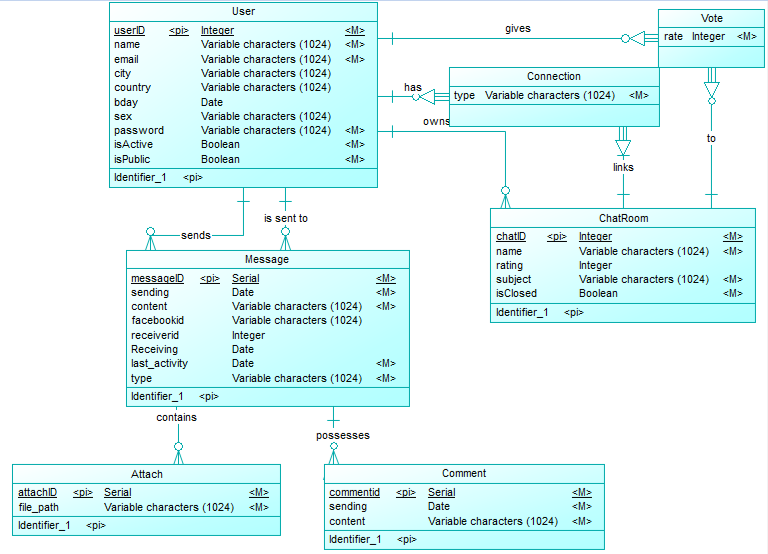
\includegraphics[keepaspectratio=true, height=0.43\textheight]{er}
	\caption{Modelo ER final.}
\end{figure}
\begin{figure}[h]
	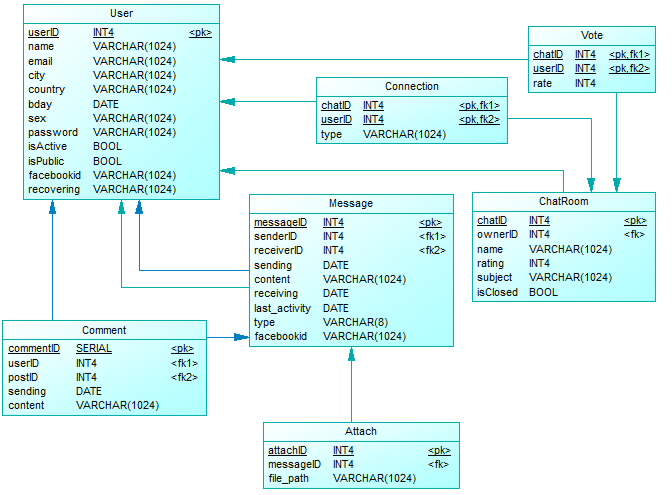
\includegraphics[keepaspectratio=true, height=0.43\textheight]{physical}
	\caption{Modelo físico final.}
\end{figure}
\cleardoublepage


\section{Scripts SQL}
\indent \indent Neste capítulo vamos explicar todos os scripts de sql que foram usados durante todo o projecto.

\subsection{Create Tables}
\indent \indent A primeira versão deste script foi auto gerada a partir do PowerDesigner quando se fez a primeira versão do modelo físico. Ao longo de todo o processo de desenvolvimento o ficheiro foi sendo alterado conforme se achou necessário. Alguns campos foram suprimidos e outros adicionados, assim como algumas constraints.

O script completo pode ser consultado em anexo.

\subsection{PL PG SQL}
\indent \indent Uma vez que a aula prática relativa a esta matéria foi bastante perto da deadline do projecto de Sistemas Distribuidos, acabaram por se resolver, com comandos SQL inseridos à mão chamados através do Java, algumas situações que normalmente seriam resolvidas com triggers, tais como o apagar de um post implica apagar todos os seus comentários, tal como todos os anexos que a ele estão associados, por uma questão de consistência de base de dados.

Assim acabámos por criar apenas um trigger e uma function. O nosso trigger dispara quando existe um insert ou um update na tabela de votos e chama a função que recalcula o rating dessa mesma chatroom.
\cleardoublepage


\section{Segurança e Integridade}
\subsection{Concorrência}
\indent \indent Tal como sugerido no enunciado tratámos da concorrência no voto. Existe uma série de regras para votar na chatroom:
\begin{itemize}
	\item Qualquer utilizador pode votar.
	\item Não podem haver mais votos do que utilizadores diferentes a comentar.
\end{itemize}

Assim como precisamos de garantir o acesso em exclusão mútua à tabela vote enquanto estamos a calcular o número de votos existentes, para aferir se um utilizador ainda ou não votar, fazemos lock à table de voto libertando-o quando terminamos a transação que está a correr naquele momento.

\subsection{Transacções}
\indent \indent Sempre que é necessário executar mais que um comando SQL para garantir que todo o processo decorre sem erros, é iniciada uma transacção com o respectivo BEGIN e é terminada com COMMIT no caso de ser bem sucedida ou com ROLLBACK no caso de se verificar um erro.

Um exemplo disto mesmo é os posts ou mensagens com anexos. É iniciada uma transacção para inserir primeiro o post e depois todos os anexos até que se chegue ao último, caso isto se verifique faz-se COMMIT, caso exista algum erro é feito ROLLBACK e nada é adicionado à base de dados.

Tal como foi referido anteriormente para fazer lock a tabelas é necessário ter uma transacção a correr, por isso também são usadas para esse efeito.
\cleardoublepage

\subsection{Segurança}
\indent \indent Para garantir a segurança das passwords dos utilizadores estas são encriptadas através do algoritmo MD5.

Nas sessões de Facebook estamos a ir buscar um access token gerado pelo próprio Facebook para termos permissões de acesso à conta, sendo que esse token apenas é válido para o id da nossa aplicação que não se encontra visivel.

Tal como dito antes, todos os forms estão preparados para não existir SQL Injection, tal como para não existir scripts a serem executados.
\cleardoublepage

\section{Gestão do Espaço}
\indent \indent Actualizando os cálculos inicialmente feitos para os novos tamanhos de tabelas, podemos ver que o acréscimo não foi muito grande.
\begin{center}
    \begin{tabular}{|p{4cm} | p{4cm} | p{4cm} |} \hline
        \textbf{Tabela}          &   \textbf{Número de Registos}      &   \textbf{Tamanho(KB)} \\ \hline
        Attach          &          300              &    1200       \\ \hline
        Comment         &          1200             &    1440       \\ \hline
        Chatroom        &          100              &    3000       \\ \hline
        Connection      &          2000             &    4000       \\ \hline
        Message         &          5000             &   10500       \\ \hline
        Users           &          1000             &    9000       \\ \hline
        Vote            &          1100             &      13       \\ \hline
        TOTAL           &        \------            &   29153       \\ \hline
    \end{tabular}
\end{center}

\subsection{PCT Free e PCT Used}
\indent \indent Segundo conseguimos apurar os parâmetros \href{http://www-2.cs.cmu.edu/~pmerson/docs/OracleToPostgres.pdf}{pctfree e pctused não existem em PostgreSQL}. De qualquer modo "assumimos" que estávamos a usar Oracle e fizemos os cálculos explicando-os de seguida.

\subsubsection{Modificações nas Tabelas}
\begin{center}
    \begin{tabular}{|p{4cm} | p{4cm} | p{4cm} |} \hline
        \textbf{Tabela}          &   \textbf{Inserções}      &   \textbf{Alterações}       \\ \hline
        Attach          &     Frequente    &   Nunca            \\ \hline
        Comment         &   Muito Frequente&   Nunca            \\ \hline
        Chatroom        &   Frequente      &   Pouco Frequente  \\ \hline
        Connection      &   Frequente      &   Pouco Frequente  \\ \hline
        Message         &   Muito Frequetne&   Nunca            \\ \hline
        Users           &   Pouco Frequente&   Frequente        \\ \hline
        Vote            &   Pouco Frequente&   Pouco Frequente  \\ \hline
    \end{tabular}
\end{center}

Como a entidade que ocupa mais espaço é o Users, com cerca de 9KB, os blocos de dados de dados poderiam ter 16KB.

\subsubsection{Attach}
\indent \indent Como esta tabela tem uma frequência de alterações nula e uma frequência de inserções frequente, podemos defenir que o PCTFREE fica a 0\%, uma vez que não vai sofrer alterações e o PCTUSED a 90\%.

\subsubsection{Comment}
\indent \indent Como esta tabela tem uma frequência de alterações nula e uma frequência de inserções muito frequente, podemos defenir que o PCTFREE fica a 0\%, uma vez que não vai sofrer alterações e o PCTUSED a 70\%.

\subsubsection{Chatroom}
\indent \indent Como esta tabela tem uma frequência de alterações pouco frequente e uma frequência de inserções frequente, podemos defenir que o PCTFREE fica a 20\%, e o PCTUSED a 80\%.

\subsubsection{Connection}
\indent \indent Como esta tabela tem uma frequência de alterações pouco frequente e uma frequência de inserções frequente, podemos defenir que o PCTFREE fica a 20\%, e o PCTUSED a 80\%. 

\subsubsection{Message}
\indent \indent Como esta tabela tem uma frequência de alterações nula e uma frequência de inserções frequente, podemos defenir que o PCTFREE fica a 0\%, uma vez que não vai sofrer alterações e o PCTUSED a 70\%. 

\subsubsection{Users}
\indent \indent Como esta tabela tem uma frequência de alterações frequente e uma frequência de inserções pouco frequente, podemos defenir que o PCTFREE fica a 30\%, e o PCTUSED a 90\%.

\subsubsection{Vote}
\indent \indent Como esta tabela tem uma frequência de alterações pouco frequente e uma frequência de inserções pouco frequente, podemos defenir que o PCTFREE fica a 20\%, e o PCTUSED a 90\%.
\cleardoublepage


\section{Indíces}
\indent \indent Para além de um índice para cada uma das chaves primárias que o Postgres cria por defeito, foram ainda criados os seguintes indíces:
\begin{itemize}
    \item CONTAINS\_FK torna mais rápidas as pesquisas de anexos a partir do messageid;
    \item OWNS\_FK torna mais rápida a pesquisa pelo owner da chatroom;
    \item EMAIL torna mais rápida a pesquisa por email, este é dos mais utilizados uma vez que o login é feito por email.
\end{itemize}

A criação destas e de todas as outras encontra-se nos anexos juntamente com a criação das tabelas.
\cleardoublepage


\section{Integração com SGBD}
\indent \indent Tal como foi dito anteriormente este projecto é a continuação do projecto de Sistemas Distribuídos pelo o website comunica com o servidor através de RMI, sendo que esse comunica com a base de dados.

\begin{figure}[h]
    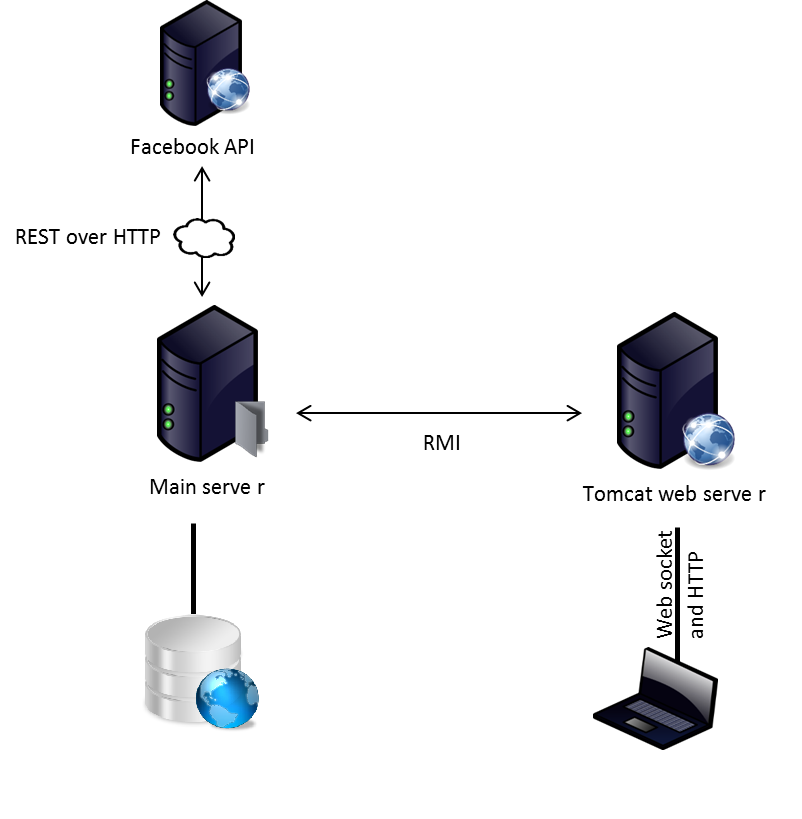
\includegraphics[keepaspectratio=true, height=0.7\textheight]{arch}
    \caption{Arquitectura da aplicação.}
\end{figure}
\cleardoublepage


\section{Testes}
\begin{center}
    \begin{tabular}{| c | p{5cm} | p{9cm} |} \hline
        \-- &   \textbf{Teste}                          &   \textbf{Resultado}\\ \hline
        1.  &   Acede à página                          &   É apresentado a página de login\\ \hline
        2.  &   Login com credenciais inválidas         &   Login falhado, continua na mesma página\\ \hline
        3.  &   Login com Facebook, 1ª vez              &   É redireccionado para a página de do facebook para autorizar a aplicação e dp de volta para a página já logged in.\\ \hline
        4.  &   Login com Facebook                      &   É automaticamente logged in.\\ \hline
        5.  &   Login com credenciais válidas           &   É logged in.\\ \hline
        6.  &   Recuperação de password                 &   É enviado um email com um website para visitar.\\ \hline
        7.  &   Visita o website de recuperação         &   É mostrado um form para preencher com a nova password.\\ \hline
        8.  &   Já logged in cria um post               &   O post é criado, caso seja um utilizador logged in pelo Facebook, o post é criado também lá.\\ \hline
        9.  &   Faz um comentário                       &   O comentário é mostrado, caso o post seja de um facebook user e o user que comentou seja amigo desse user, o comment vai também ele para o Facebook.\\ \hline
        10. &   Criar um post com anexos                &   O post é criado e os anexos mostrados.\\ \hline
        11. &   Ir para o menu de mensagens privadas    &   É mostrado um resumo de todas as ultimas mensagens trocadas com todos os utilizadores. As mensagens que ainda não foram lidas são destacadas.\\ \hline
        12. &   Criar uma mensagem                      &   A mensagem é criada e enviada.\\ \hline
        13. &   Criar uma mensagem com anexos           &   A mensagem é criada com os anexos.\\ \hline
        14. &   Criar uma mensagem delayed              &   A mensagem só é mostrada na altura certa. O utilizador só a vê quando actualiza a página.\\ \hline
    \end{tabular}
\end{center}
\cleardoublepage
\begin{center}
    \begin{tabular}{| c | p{5cm} | p{9cm} |} \hline
        \-- &   \textbf{Teste}                          &   \textbf{Resultado}\\ \hline
        15. &   Ir para o menu de chatrooms             &   É apresentado um menu com as oito categorias.\\ \hline
        16. &   Escolher uma categoria                  &   É apresentada uma lista de chatrooms pertecentes aquela categoria.\\ \hline
        17. &   Escolher uma dessas chatrooms           &   É aberta a página dessa chatroom.\\ \hline
        18. &   Criar uma mensagem                      &   A mensagem é criada e enviada.\\ \hline
        19. &   Criar uma mensagem com anexos           &   A mensagem é criada com os anexos.\\ \hline
        20. &   Carregar no botão de criar chatroom     &   É apresentado o formulário de criação de chatroom.\\ \hline
        21. &   Carregar no botão de editar chatroom    &   É apresentado o menu de gestão da chatroom.\\ \hline
        22. &   Votar numa chatroom                     &   Caso seja possível o voto é adicionado e é recalculado o rating da chatroom.\\ \hline
        23. &   No histórico de private messages apagar &   É apresentado um botão junto à hora que permite ao utilizador apagar mensagens que ainda não tenham sido lidas.\\ \hline
        24. &   Carregar no nome de um utilizador       &   É redireccionado para a página do utilizador onde é mostrada a informação desse utilizador, os seus posts, e as chatrooms que criou.\\ \hline
        25. &   Na wall editar um post                  &   O texto do post fica editável.\\ \hline
        26. &   Na wall apagar um post                  &   É mostrado um ecrã de confirmação para apagar o post.\\ \hline
        27. &   No meu perfil carregar em editar        &   Os dados do utilizador ficam editáveis.\\ \hline
        28. &   No meu perfil carregar em cancelar conta&   É mostrado um ecrã de confirmação de cancelamento.\\ \hline
    \end{tabular}
\end{center}
\cleardoublepage

\section{Gestão do Projecto}
\begin{center}
    \begin{tabular}{| c | p{8cm} | p{6cm} |} \hline
        \-- &   \textbf{Tarefa}                             &   \textbf{Encarregado}\\ \hline
        1.  &   Definição do sistema e das Funcionalidades  &   Alexandre Santos e João Ferreira\\ \hline
        2.  &   Diagrama ER                                 &   João Ferreira\\ \hline
        3.  &   Diagrama Físico                             &   João Ferreira\\ \hline
        4.  &   Criação de procedures e triggers            &   João Ferreira\\ \hline
        5.  &   Criação de índices                          &   Alexandre Santos\\ \hline
        6.  &   Ligação entre o sistema e a base de dados   &   Alexandre Santos\\ \hline
        7.  &   Criação da interface do website             &   Alexandre Santos\\ \hline
        8.  &   Implementação de funcionalidades no website &   Alexandre Santos\\ \hline
        9.  &   População da base de dados                  &   Alexandre Santos e João Ferreira\\ \hline
        10. &   Testes ao sistema                           &   Alexandre Santos e João Ferreira\\ \hline
        11. &   Correcção de erros no sistema               &   Alexandre Santos e João Ferreira\\ \hline
        12. &   Documentação das várias metas do projecto   &   João Ferreira\\ \hline
        13. &   Integração com o Facebook                   &   Alexandre Santos e João Ferreira\\ \hline
        14. &   Integração com o Serviços de Email          &   Alexandre Santos e João Ferreira\\ \hline
        15. &   Protecção contra SQL Injection              &   João Ferreira\\ \hline
        16. &   Interface do website                        &   Alexandre Santos\\ \hline
    \end{tabular}
\end{center}
\cleardoublepage


\section{Conclusão}
\indent \indent Apesar de não ter havido disponibilidade para implementar algumas funcionalidades extra que se gostaria de ter implementado, as funcionalidades que tinham sido propostas implementar no início do projecto foram cumpridas e foram ainda acrescentadas outras que pareceram pertinentes.

Considera-se que o projecto foi bem sucedido uma vez que foram tratados os principais pontos da criação / gestão de uma base de dados: o seu planeamento, a criação e actualização dos diagramas ER e físicos, a geração de tabelas e scripts, a integridade da base de dados, transacções e concorrência e a criação de índices para díminuir o tempo de pesquisa.
\cleardoublepage

\section{Anexos}
\subsection{Criação das Tabelas}
\begin{verbatim}
/*==============================================================*/
/* DBMS name:      PostgreSQL 8                                 */
/* Created on:     11/6/2012 5:21:26 PM                         */
/*==============================================================*/

/*==============================================================*/
/* Table: ATTACH                                                */
/*==============================================================*/
create table ATTACH (
   ATTACHID             SERIAL               not null,
   MESSAGEID            INT4                 not null,
   FILE_PATH            VARCHAR(1024)        not null,
   constraint PK_ATTACH primary key (ATTACHID)
);

/*==============================================================*/
/* Index: ATTACH_PK                                             */
/*==============================================================*/
create unique index ATTACH_PK on ATTACH (
ATTACHID
);
\end{verbatim}
\cleardoublepage
\begin{verbatim}
/*==============================================================*/
/* Table: COMMENT                                               */
/*==============================================================*/
create table COMMENT (
   COMMENTID            SERIAL               not null,
   POSTID               INT4                 not null,
   USERID               INT4                 not null,
   SENDING              TIMESTAMP            not null,
   CONTENT              VARCHAR(1024)        not null,
   constraint PK_COMMENT primary key (COMMENTID)
);

/*==============================================================*/
/* Index: POSTCOMMENT_PK                                        */
/*==============================================================*/
create index POSTCOMMENT_PK on COMMENT (
POSTID
);

/*==============================================================*/
/* Index: CONTAINS_FK                                           */
/*==============================================================*/
create  index CONTAINS_FK on ATTACH (
MESSAGEID
);
\end{verbatim}
\cleardoublepage
\begin{verbatim}
/*==============================================================*/
/* Table: CHATROOM                                              */
/*==============================================================*/
create table CHATROOM (
   CHATID               SERIAL               not null,
   OWNERID              INT4                 not null,
   NAME                 VARCHAR(1024)        not null,
   RATING               INT4                 null,
   SUBJECT              VARCHAR(1024)        not null,
   ISCLOSED             BOOL                 not null,
   constraint PK_CHATROOM primary key (CHATID),
   constraint subject_type CHECK (SUBJECT IN ('economia','mundo','cultura',
   'desporto','ciencia','tecnologia','multimedia','musica'))
);

/*==============================================================*/
/* Index: CHATROOM_PK                                           */
/*==============================================================*/
create unique index CHATROOM_PK on CHATROOM (
CHATID
);

/*==============================================================*/
/* Index: OWNS_FK                                               */
/*==============================================================*/
create  index OWNS_FK on CHATROOM (
OWNERID
);
\end{verbatim}
\cleardoublepage
\begin{verbatim}
/*==============================================================*/
/* Table: CONNECTION                                            */
/*==============================================================*/
create table CONNECTION (
   CHATID               INT4                 not null,
   USERID               INT4                 not null,
   TYPE                 VARCHAR(1024)        not null,
   constraint PK_CONNECTION primary key (CHATID, USERID),
   constraint message_type CHECK (type IN ('poster','watcher'))
);

/*==============================================================*/
/* Index: CONNECTION_PK                                         */
/*==============================================================*/
create unique index CONNECTION_PK on CONNECTION (
CHATID,
USERID
);

/*==============================================================*/
/* Index: LINKS_FK                                              */
/*==============================================================*/
create  index LINKS_FK on CONNECTION (
CHATID
);

/*==============================================================*/
/* Index: HAS_FK                                                */
/*==============================================================*/
create  index HAS_FK on CONNECTION (
USERID
);
\end{verbatim}
\cleardoublepage
\begin{verbatim}
/*==============================================================*/
/* Table: MESSAGE                                               */
/*==============================================================*/
create table MESSAGE (
   MESSAGEID            SERIAL               not null,
   FACEBOOKID           VARCHAR(1024)        null,
   SENDERID             INT4                 not null,
   SENDING              TIMESTAMP            not null,
   CONTENT              VARCHAR(1024)        not null,
   RECEIVERID           INT4                 null,
   RECEIVING            TIMESTAMP            null,
   LAST_ACTIVITY        TIMESTAMP            not null,
   TYPE                 VARCHAR(8)           not null,
   constraint PK_MESSAGE primary key (MESSAGEID),
   constraint message_type CHECK (type IN ('public','private','post'))
);

/*==============================================================*/
/* Index: MESSAGE_PK                                            */
/*==============================================================*/
create unique index MESSAGE_PK on MESSAGE (
MESSAGEID
);
\end{verbatim}
\cleardoublepage
\begin{verbatim}
/*==============================================================*/
/* Table: USERS                                                */
/*==============================================================*/
create table USERS (
   USERID               SERIAL               not null,
   NAME                 VARCHAR(1024)        not null,
   EMAIL                VARCHAR(1024)        not null,
   FACEBOOKID           VARCHAR(1024)        null,
   CITY                 VARCHAR(1024)        null,
   COUNTRY              VARCHAR(1024)        null,
   BDAY                 DATE                 null,
   SEX                  VARCHAR(1024)        null,
   RECOVERING           VARCHAR(1024)        null,
   PASSWORD             VARCHAR(1024)        not null,
   ISACTIVE             BOOL                 not null,
   ISPUBLIC             BOOL                 not null,
   constraint PK_USER primary key (USERID),
   constraint ID_EMAIL unique (EMAIL),
);

/*==============================================================*/
/* Index: USER_PK                                               */
/*==============================================================*/
create unique index USER_PK on USERS (
USERID
);

/*==============================================================*/
/* Index: EMAIL                                                 */
/*==============================================================*/
create unique index EMAIL on USERS (
EMAIL
);
\end{verbatim}
\cleardoublepage
\begin{verbatim}
/*==============================================================*/
/* Table: VOTE                                                  */
/*==============================================================*/
create table VOTE (
   CHATID               INT4                 not null,
   USERID               INT4                 not null,
   RATE                 INT4                 not null,
   constraint PK_VOTE primary key (CHATID, USERID),
   constraint vote_rate CHECK (rate IN (1, 2, 3))
);

/*==============================================================*/
/* Index: VOTE_PK                                               */
/*==============================================================*/
create unique index VOTE_PK on VOTE (
CHATID,
USERID
);

/*==============================================================*/
/* Index: TO_FK                                                 */
/*==============================================================*/
create  index TO_FK on VOTE (
CHATID
);

/*==============================================================*/
/* Index: GIVES_FK                                              */
/*==============================================================*/
create  index GIVES_FK on VOTE (
USERID
);
\end{verbatim}
\cleardoublepage
\begin{verbatim}
alter table ATTACH
   add constraint FK_ATTACH_CONTAINS_MESSAGE foreign key (MESSAGEID)
      references MESSAGE (MESSAGEID)
      on delete restrict on update restrict;

alter table CHATROOM
   add constraint FK_CHATROOM_OWNS_USER foreign key (OWNERID)
      references USERS (USERID)
      on delete restrict on update restrict;

alter table CONNECTION
   add constraint FK_CONNECTI_HAS_USER foreign key (USERID)
      references USERS (USERID)
      on delete restrict on update restrict;

alter table CONNECTION
   add constraint FK_CONNECTI_LINKS_CHATROOM foreign key (CHATID)
      references CHATROOM (CHATID)
      on delete restrict on update restrict;

alter table MESSAGE
   add constraint FK_MESSAGE_SENDS_USER foreign key (SENDERID)
      references USERS (USERID)
      on delete restrict on update restrict;

alter table VOTE
   add constraint FK_VOTE_GIVES_USER foreign key (USERID)
      references USERS (USERID)
      on delete restrict on update restrict;

alter table VOTE
   add constraint FK_VOTE_TO_CHATROOM foreign key (CHATID)
      references CHATROOM (CHATID)
      on delete restrict on update restrict;
\end{verbatim}
\cleardoublepage

\subsection{Trigger e Function}
\begin{verbatim}
create or replace function calcRating() returns trigger as $$
declare
    c cursor is
        select rate from vote where chatid = NEW.chatid;
    sum decimal := 0;
    rate chatroom.rating % type;
begin
    open c;
    loop
        fetch c into rate;
        exit when not found;
        sum := sum + rate;
    end loop;
    sum := sum / (select count(*) from vote where chatid = NEW.CHATID);
    update chatroom set rating = round(sum, 0) where chatid = NEW.CHATID;
    return null;
end;
$$ language plpgsql;

CREATE TRIGGER updateRating
    AFTER INSERT OR UPDATE ON vote
    FOR EACH ROW
    EXECUTE PROCEDURE calcRating();

\end{verbatim}
\end{document}
